\documentclass[11pt,letterpaper]{article}
\usepackage[T1]{fontenc}
\usepackage{lmodern}
\usepackage[margin=1in,headheight=15pt]{geometry}
\usepackage{amsmath,amssymb,bm,mathtools}
\usepackage{microtype}
\usepackage{booktabs,array,tabularx,longtable}
\usepackage{enumitem,needspace}
\usepackage{tikz,pgfplots}
\usetikzlibrary{arrows.meta,calc}
\usepgfplotslibrary{groupplots}
\pgfplotsset{compat=1.18}
\usepackage{listings}
\usepackage{fancyhdr,xcolor}
\definecolor{linkblue}{RGB}{29,62,96}
\definecolor{lightgray}{RGB}{245,246,247}
\usepackage[colorlinks=true,linkcolor=linkblue,citecolor=linkblue,urlcolor=linkblue,menucolor=linkblue]{hyperref}
\hypersetup{pdftitle={Fixed-Pivot Roller Flyweights: Geometry, Mass and the Common Boundary},pdfauthor={CINDER technical note},pdfsubject={Construction and verification of a centrifugal mechanism through effective mass and shaft inertia}}
\usepackage[nameinlink,noabbrev]{cleveref}
\setlength{\parindent}{0pt}
\setlength{\parskip}{0.55em}
\setlength{\emergencystretch}{2em}
\clubpenalty=10000
\widowpenalty=10000
\setlist{topsep=.3em,itemsep=.3em,parsep=0pt}
\numberwithin{equation}{section}
\pagestyle{fancy}
\fancyhf{}
\fancyhead[L]{\small CINDER \enspace / \enspace Clamping mechanism implementations}
\fancyhead[R]{\small CINDER 1.2.0}
\fancyfoot[L]{\small\Acrobatmenu{GoBack}{Previous view}}
\fancyfoot[C]{\thepage}
\fancyfoot[R]{\small\hyperlink{note-contents}{Contents}}
\renewcommand{\headrulewidth}{.3pt}
\lstset{language=Python,basicstyle=\small\ttfamily,keywordstyle=\color{linkblue},commentstyle=\itshape\color{gray},backgroundcolor=\color{lightgray},frame=single,framerule=.3pt,rulecolor=\color{gray},columns=fullflexible,keepspaces=true,showstringspaces=false,breaklines=true,aboveskip=.8em,belowskip=.8em}
\newcommand{\dd}{\mathrm{d}}
\newcommand{\half}{\tfrac12}
\newcommand{\e}{\bm e}
\newcommand{\term}[1]{\par\needspace{4\baselineskip}\textbf{#1}\enspace}
\newcolumntype{Y}{>{\raggedright\arraybackslash}X}
\newcolumntype{P}[1]{>{\raggedright\arraybackslash}p{#1}}

\begin{document}
\thispagestyle{plain}
\begin{center}
{\small CINDER TECHNICAL NOTE \quad $\cdot$ \quad CINDER 1.2.0 \quad $\cdot$ \quad OCTOBER 11, 2026}
\vspace{.7em}

{\LARGE\bfseries Clamping Mechanism Implementations\par}
\vspace{.45em}
{\large Part I: The Fixed-Pivot Roller Flyweight\par}
\end{center}
\vspace{.4em}

The general centrifugal-mechanism derivation \cite{general} identifies the quantities needed at the boundary to the surrounding CVT: an effective mass $M_f(x)$ for sheave motion, a shaft-axis inertia $J_f(x)$, and their position derivatives. A particular mechanism must still supply those quantities from its attachments, contact geometry, and mass distribution. That construction is the subject of this document.

We begin with the fixed-pivot roller flyweight already used in CINDER. Its known force law makes it a useful first test: constructing the new maps must recover the existing mechanics, including shaft coupling and kinetic energy. The derivation follows the physical assembly from the ramp surface to the roller pose, then from the motion of the retained mass to the four returned quantities. The assumptions are stated before they are used.

The manuscript reference is the October 1, 2026 formulation \cite{formulation}, especially Section 3.2.1 and Appendix A. The numerical reference is CINDER v1.1.5 \cite{implementation}; the preserved companion reconstructs that mechanism independently. CINDER 1.2.0 now routes this same runtime map through the canonical four-quantity boundary. The separate sliding-block document states its own attachments and assumptions; the two mechanisms share the boundary, not their contact construction.

\hypertarget{note-contents}{}
\begingroup\small\setlength{\parskip}{0pt}
\setcounter{tocdepth}{1}\tableofcontents
\endgroup\clearpage
\section{The boundary each implementation must supply}
\label{sec:boundary}

Let $x$ be local movable-sheave displacement, positive in the closing direction, and let $\omega$ and $\alpha=\dot\omega$ be shaft angular speed and acceleration. A prime denotes differentiation with respect to $x$. For the mechanism class considered here, the internal configuration is determined by $x$, and the retained kinetic energy is
\begin{equation}
  T_f=\half M_f(x)\dot x^2+\half J_f(x)\omega^2.
  \label{eq:energy}
\end{equation}
There is no retained mixed term $B_f(x)\omega\dot x$. The symmetry assumption that makes this true for the present flyweight will be stated explicitly below.

At any admitted position, the mechanism supplies
\begin{equation}
  \mathcal I_f(x)=\bigl(M_f(x),\ M_f'(x),\ J_f(x),\ J_f'(x)\bigr).
  \label{eq:payload}
\end{equation}
The quantities have units $\mathrm{kg}$, $\mathrm{kg\,m^{-1}}$, $\mathrm{kg\,m^2}$, and $\mathrm{kg\,m}$, respectively. They are two functions and their derivatives, not four independent force fits. The common mechanical relations are
\begin{align}
  F_{f,x}&=\half J_f'\omega^2-M_f\ddot x-\half M_f'\dot x^2,
       \label{eq:force}\\
  \tau_f&=-J_f\alpha-J_f'\dot x\omega.
       \label{eq:torque}
\end{align}
Here $F_{f,x}$ is the net closing force delivered to the movable assembly, and $\tau_f$ is the reaction torque delivered to the shaft. Their derivation and power identity are given in \cite{general}; both relations are retained in this implementation.

On the admitted interval, $M_f$ and $J_f$ must be finite and nonnegative. Taking them to be $C^1$, with their actual derivatives returned in \cref{eq:payload}, makes these force and torque coefficients continuous. The regularity needed by the underlying geometry is established as part of the construction below.

The geometry routine may use angles, contact coordinates, and detailed mass moments internally. It need not expose those variables to the common force law. Conversely, the four inertia quantities do not describe the shape of a ramp or the reactions at individual contacts. The implementation also retains its valid travel interval and a mechanism-specific contact check. Springs and belt reactions remain separate loads in the surrounding pulley balances.

\section{Mechanism I: what is attached to what?}
\label{sec:assembly}

The flyweight pivot is attached to the shaft-fixed pulley body. The ramp is carried by the movable sheave and translates as that sheave closes. A rigid arm places the centre of a circular roller a fixed distance from the pivot. As the ramp translates beneath the roller, the contact geometry determines the arm's angle. The pivot stays fixed in the shaft frame, even though the entire assembly rotates with the shaft.

This attachment pattern matters mechanically. The ramp contact loads the movable assembly, while the pivot reaction is carried by the shaft-fixed body. There is no additional axial work at the pivot during a virtual sheave displacement. A mechanism with a translating pivot would have a different load path and a different effective mass, even if it produced the same radial motion of its weights.

\subsection{Physical assumptions for this mechanism}

The following assumptions define the fixed-pivot model used throughout this part. The separate mass approximation and numerical approximation are stated later so that they are not mistaken for consequences of these assumptions.

\begin{longtable}{@{}p{.07\textwidth}p{.85\textwidth}@{}}
\toprule
 & Assumption and its consequence\\
\midrule
\endhead
F1 & \textbf{Fixed pivot and translating ramp.} Each pivot is fixed in the shaft frame; its ramp undergoes rigid axial translation by $x$. The arm angle is therefore determined by their relative geometry.\\[.5em]
F2 & \textbf{Rigid arm and circular roller.} The pivot-to-centre distance and roller radius are constant. Elastic changes of the arm, ramp, and contact patch are omitted.\\[.5em]
F3 & \textbf{Planar relative motion.} The arm and roller centre move in an axial--radial section. Out-of-plane deflection and a separate internal positional degree of freedom are omitted.\\[.5em]
F4 & \textbf{Mass symmetry sufficient to remove mixed coupling.} Each represented mass distribution is symmetric about its axial--radial plane, or its omitted cross moments cancel in the complete set. Repetition around the shaft alone is not sufficient to establish this condition.\\[.5em]
F5 & \textbf{Identical repeated flyweights.} The $n_f$ members have the same geometry, selected pose, and mass moments. Their inertia contributions add, and the ideal symmetric loading gives equal roller reactions.\\[.5em]
F6 & \textbf{Ideal contact and pivot.} Ramp contact transmits only a normal reaction. Pivot friction, bearing loss, guide friction, backlash, clearance, and local damping are omitted. No rolling-speed constraint or roller-spin state is introduced.\\[.5em]
F7 & \textbf{One active roller--ramp contact per member.} The selected contact is maintained while its required normal reaction is nonnegative. Flyweight lift-off, re-impact, and simultaneous contact with two ramp locations are outside this branch.\\[.5em]
F8 & \textbf{A fixed retained mass set and no other mechanism load.} The chosen bodies retain constant mass. Their mass and inertia are not counted again in the rigid sheave or fixed pulley quantities. Springs, gravity if retained, and other applied loads require separate terms.\\
\bottomrule
\end{longtable}

F6 does not set the roller radius to zero. A roller can have a finite geometric radius while its spin dynamics are omitted. Whether its finite size also contributes to the mass moments is a separate modelling decision, addressed in \cref{sec:mass-approx}.

\subsection{Requirements on the selected branch}

These assumptions do not guarantee that every proposed geometry can operate over every travel interval. The selected branch must exist throughout the declared range, remain regular, and avoid interference. To reproduce the existing CINDER mechanism, it must give finite $q_f'(x)>0$, finite $q_f''(x)$, and a normal reaction whose projection onto the movable assembly is in the closing direction. The geometric tests establish a usable configuration map; the normal-force test must still be performed using the solved acceleration.

\section{Constructing the roller contact from the physical ramp}
\label{sec:geometry}

Use $X$ for the physical axial coordinate of a point, to distinguish it from the sheave displacement $x$. Let $r$ be its radial coordinate. In the shaft frame, the pivot is
\begin{equation}
  P=(X_P,r_P).
\end{equation}
Let $L_f$ be the rigid pivot-to-roller-centre distance, $R_{\mathrm{roll}}$ the roller radius, and $q_f$ the arm angle measured from the positive axial direction toward the radial direction. If $C$ is the roller centre, then
\begin{equation}
  \bm c(q_f)=
  \begin{bmatrix}X_P\\r_P\end{bmatrix}
  +L_f\begin{bmatrix}\cos q_f\\\sin q_f\end{bmatrix}.
  \label{eq:arm-circle}
\end{equation}
The arm restricts the roller centre to a circle. The ramp imposes a second restriction; their intersection determines the pose.

\subsection{The surface and its normal}

Let $\xi$ be a ramp coordinate with units of length, and let $h(\xi)$ be the ramp's radial height above its reference point $A=(X_A,r_A)$ at zero closure. The physical contact point $K$ has position
\begin{equation}
  \bm k(\xi,x)=
  \begin{bmatrix}X_A+x+d\xi\\r_A+h(\xi)\end{bmatrix},
  \qquad d\in\{-1,+1\}.
  \label{eq:surface}
\end{equation}
The direction $d$ specifies which way increasing $\xi$ proceeds axially. The reference implementation uses $d=-1$: increasing $\xi$ walks toward the pivot while the ramp rises radially.

Define the profile derivatives and tangent length by
\begin{equation}
  p=h_{\xi},\qquad k=h_{\xi\xi},\qquad t=h_{\xi\xi\xi},
  \qquad w=\sqrt{1+p^2}.
\end{equation}
Subscripts $\xi$ here denote profile-coordinate derivatives; primes below continue to mean derivatives with respect to sheave travel $x$. The tangent and selected unit normal are
\begin{equation}
  \bm t_0=\begin{bmatrix}d\\p\end{bmatrix},
  \qquad
  \bm n=\frac{\sigma}{w}\begin{bmatrix}-p\\d\end{bmatrix},
  \qquad \sigma\in\{-1,+1\}.
  \label{eq:normal}
\end{equation}
The sign $\sigma$ selects the physical side of the ramp carrying the roller. It is fixed by the assembly and is not changed merely to make a computed reaction positive.

\subsection{The roller centre is an offset curve}

The physical ramp is touched by the roller surface, not by its centre. Consequently the compatible roller-centre location is
\begin{equation}
  \bm c(\xi,x)=\bm k(\xi,x)+R_{\mathrm{roll}}\bm n(\xi).
  \label{eq:offset}
\end{equation}
Figure~\ref{fig:geometry} shows the distinction. Replacing $\bm c$ by $\bm k$ would change both the assembled angle and its derivatives. It would be a point-follower approximation, rather than an alternative implementation of the finite-roller model.

\begin{figure}[htbp]
\centering
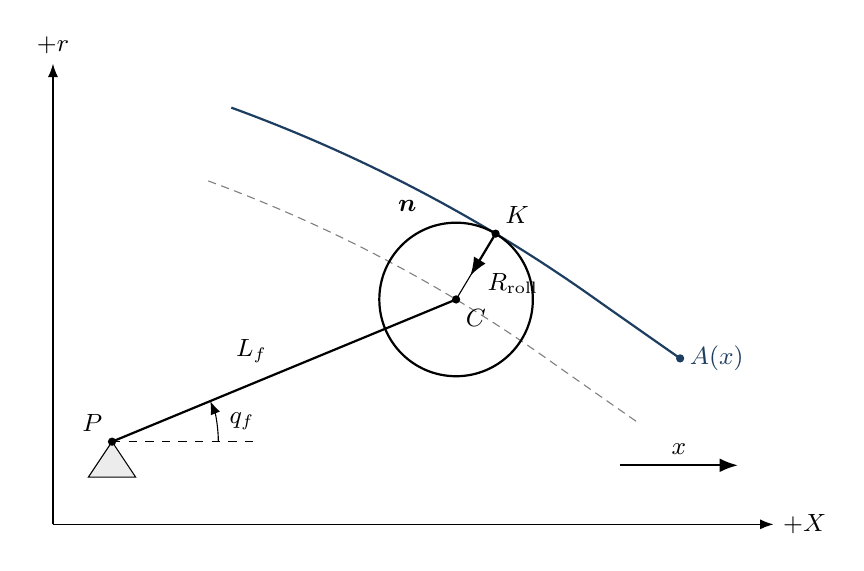
\begin{tikzpicture}[x=.15cm,y=.15cm,>=Latex,font=\small]
\draw[->] (-5,-7)--(56,-7) node[right] {$+X$};
\draw[->] (-5,-7)--(-5,32) node[above] {$+r$};
\draw[thick,linkblue] plot coordinates {(48.1000000,7.0510400) (47.7833333,7.2727724) (47.4666667,7.4945048) (47.1500000,7.7162372) (46.8333333,7.9379695) (46.5166667,8.1597019) (46.2000000,8.3814343) (45.8833333,8.6031667) (45.5666667,8.8248991) (45.2500000,9.0466315) (44.9333333,9.2683639) (44.6166667,9.4900963) (44.3000000,9.7118286) (43.9833333,9.9335610) (43.6666667,10.1552934) (43.3500000,10.3770258) (43.0333333,10.5987582) (42.7166667,10.8205187) (42.4000000,11.0424873) (42.0833333,11.2649337) (41.7666667,11.4880531) (41.4500000,11.7118568) (41.1333333,11.9361283) (40.8166667,12.1604417) (40.5000000,12.3842442) (40.1833333,12.6070017) (39.8666667,12.8284011) (39.5500000,13.0483989) (39.2333333,13.2670037) (38.9166667,13.4842240) (38.6000000,13.7000683) (38.2833333,13.9145448) (37.9666667,14.1276617) (37.6500000,14.3394271) (37.3333333,14.5498490) (37.0166667,14.7589351) (36.7000000,14.9666932) (36.3833333,15.1731310) (36.0666667,15.3782558) (35.7500000,15.5820752) (35.4333333,15.7845965) (35.1166667,15.9858268) (34.8000000,16.1857733) (34.4833333,16.3844429) (34.1666667,16.5818427) (33.8500000,16.7779793) (33.5333333,16.9728596) (33.2166667,17.1664901) (32.9000000,17.3588775) (32.5833333,17.5500282) (32.2666667,17.7399486) (31.9500000,17.9286449) (31.6333333,18.1161234) (31.3166667,18.3023902) (31.0000000,18.4874513) (30.6833333,18.6713127) (30.3666667,18.8539804) (30.0500000,19.0354601) (29.7333333,19.2157576) (29.4166667,19.3948785) (29.1000000,19.5728284) (28.7833333,19.7496128) (28.4666667,19.9252373) (28.1500000,20.0997071) (27.8333333,20.2730277) (27.5166667,20.4452042) (27.2000000,20.6162418) (26.8833333,20.7861456) (26.5666667,20.9549207) (26.2500000,21.1225721) (25.9333333,21.2891047) (25.6166667,21.4545233) (25.3000000,21.6188329) (24.9833333,21.7820380) (24.6666667,21.9441434) (24.3500000,22.1051538) (24.0333333,22.2650736) (23.7166667,22.4239075) (23.4000000,22.5816598) (23.0833333,22.7383350) (22.7666667,22.8939374) (22.4500000,23.0484713) (22.1333333,23.2019410) (21.8166667,23.3543507) (21.5000000,23.5057045) (21.1833333,23.6560064) (20.8666667,23.8052606) (20.5500000,23.9534711) (20.2333333,24.1006417) (19.9166667,24.2467765) (19.6000000,24.3918791) (19.2833333,24.5359536) (18.9666667,24.6790035) (18.6500000,24.8210326) (18.3333333,24.9620447) (18.0166667,25.1020433) (17.7000000,25.2410320) (17.3833333,25.3790143) (17.0666667,25.5159939) (16.7500000,25.6519740) (16.4333333,25.7869582) (16.1166667,25.9209498) (15.8000000,26.0539521) (15.4833333,26.1859685) (15.1666667,26.3170022) (14.8500000,26.4470564) (14.5333333,26.5761344) (14.2166667,26.7042392) (13.9000000,26.8313740) (13.5833333,26.9575419) (13.2666667,27.0827458) (12.9500000,27.2069888) (12.6333333,27.3302739) (12.3166667,27.4526039) (12.0000000,27.5739818) (11.6833333,27.6944105) (11.3666667,27.8138927) (11.0500000,27.9324312) (10.7333333,28.0500289) (10.4166667,28.1666885) (10.1000000,28.2824125)};
\draw[densely dashed,gray] plot coordinates {(44.3717532,1.7265517) (44.0550865,1.9482841) (43.7384198,2.1700165) (43.4217532,2.3917489) (43.1050865,2.6134813) (42.7884198,2.8352136) (42.4717532,3.0569460) (42.1550865,3.2786784) (41.8384198,3.5004108) (41.5217532,3.7221432) (41.2050865,3.9438756) (40.8884198,4.1656080) (40.5717532,4.3873404) (40.2550865,4.6090727) (39.9384198,4.8308051) (39.6217532,5.0525375) (39.3050801,5.2742744) (38.9874224,5.4967290) (38.6668870,5.7214096) (38.3434835,5.9485888) (38.0187994,6.1773572) (37.6952610,6.4060171) (37.3754145,6.6325403) (37.0612401,6.8550886) (36.7534786,7.0725988) (36.4509245,7.2854301) (36.1501263,7.4957350) (35.8493470,7.7046954) (35.5485676,7.9123327) (35.2477883,8.1186549) (34.9470090,8.3236702) (34.6462296,8.5273863) (34.3454503,8.7298110) (34.0446710,8.9309521) (33.7438916,9.1308169) (33.4431123,9.3294131) (33.1423330,9.5267479) (32.8415536,9.7228285) (32.5407743,9.9176622) (32.2399950,10.1112559) (31.9392156,10.3036165) (31.6384363,10.4947510) (31.3376570,10.6846661) (31.0368776,10.8733683) (30.7360983,11.0608644) (30.4353190,11.2471608) (30.1345396,11.4322638) (29.8337603,11.6161798) (29.5329810,11.7989150) (29.2322016,11.9804756) (28.9314223,12.1608675) (28.6306430,12.3400969) (28.3298637,12.5181694) (28.0290843,12.6950911) (27.7283050,12.8708677) (27.4275257,13.0455047) (27.1267463,13.2190078) (26.8259670,13.3913826) (26.5251877,13.5626344) (26.2244083,13.7327687) (25.9236290,13.9017908) (25.6228497,14.0697059) (25.3220703,14.2365192) (25.0212910,14.4022358) (24.7205117,14.5668607) (24.4197323,14.7303990) (24.1189530,14.8928556) (23.8181737,15.0542352) (23.5173943,15.2145428) (23.2166150,15.3737831) (22.9158357,15.5319606) (22.6150563,15.6890801) (22.3142770,15.8451461) (22.0134977,16.0001632) (21.7127183,16.1541357) (21.4119390,16.3070681) (21.1111597,16.4589647) (20.8103803,16.6098297) (20.5096010,16.7596675) (20.2088217,16.9084822) (19.9080424,17.0562780) (19.6072630,17.2030589) (19.3064837,17.3488289) (19.0057044,17.4935921) (18.7049250,17.6373524) (18.4041457,17.7801136) (18.1033664,17.9218797) (17.8025870,18.0626544) (17.5018077,18.2024414) (17.2010284,18.3412444) (16.9002490,18.4790672) (16.5994697,18.6159134) (16.2986904,18.7517864) (15.9979110,18.8866899) (15.6971317,19.0206273) (15.3963524,19.1536021) (15.0955730,19.2856176) (14.7947937,19.4166773) (14.4940144,19.5467845) (14.1932350,19.6759425) (13.8924557,19.8041544) (13.5916764,19.9314236) (13.2908970,20.0577531) (12.9901177,20.1831462) (12.6893384,20.3076058) (12.3885591,20.4311352) (12.0877797,20.5537372) (11.7870004,20.6754150) (11.4862211,20.7961714) (11.1854417,20.9160093) (10.8846624,21.0349317) (10.5838831,21.1529414) (10.2831037,21.2700411) (9.9823244,21.3862338) (9.6815451,21.5015221) (9.3807657,21.6159088) (9.0799864,21.7293965) (8.7792071,21.8419880) (8.4784277,21.9536857) (8.1776484,22.0644924) (7.8768691,22.1744105)};
\coordinate (P) at (0,0);
\coordinate (C) at (29.1307845,12.0414307);
\coordinate (K) at (32.4765593,17.6142030);
\coordinate (A) at (48.1000000,7.0510400);
\draw[fill=gray!15] (P)--(-2,-3)--(2,-3)--cycle;
\draw[thick] (P)--(C) node[pos=.48,above left] {$L_f$};
\draw[thick] (C) circle[radius=6.5];
\draw[thin] (C)--(K) node[pos=.55,below right] {$R_{\mathrm{roll}}$};
\draw[->,thick] (K)--($(K)!.64!(C)$);
\node at (25,20) {$\bm n$};
\fill (P) circle[radius=.35] node[above left] {$P$};
\fill (C) circle[radius=.35] node[below right] {$C$};
\fill (K) circle[radius=.35] node[above right] {$K$};
\fill[linkblue] (A) circle[radius=.35] node[right] {$A(x)$};
\draw[dashed] (P)--(12,0);
\draw[->] (9,0) arc[start angle=0,end angle=22.4581256,radius=9];
\node at (11,1.7) {$q_f$};
\draw[->,thick] (43,-2)--(53,-2) node[midway,above] {$x$};
\end{tikzpicture}
\caption{Fixed-pivot reference geometry at $x=10\,\mathrm{mm}$. The solid curve is the physical ramp; the dashed curve is its roller-centre offset. The roller touches at $K$, while its centre $C$ lies on the arm circle. The axes indicate local directions; the shaft axis is outside this detail view.}
\label{fig:geometry}
\end{figure}

Write
\begin{equation}
  a=c_X-X_P,\qquad b=c_r-r_P.
\end{equation}
The arm constraint becomes the scalar equation
\begin{equation}
  \boxed{g(\xi,x)=a^2+b^2-L_f^2=0.}
  \label{eq:constraint}
\end{equation}
Solving it on the selected branch gives $\xi(x)$, followed by
\begin{equation}
  q_f(x)=\operatorname{atan2}(b,a).
  \label{eq:angle}
\end{equation}
There is no independently prescribed initial angle. The initial angle follows from the ramp, roller, pivot, and arm dimensions.

\term{Selecting an assembly.}
Several roots of \cref{eq:constraint} can describe different arm orientations. The existing implementation enumerates admissible configurations at the start of travel, selects the smallest-angle initial configuration, and follows that same branch continuously. Choosing the smallest root again at each position could jump between disconnected assemblies. A second mathematical orientation is not itself a second physical contact; interference occurs when the same selected roller pose also touches or penetrates another part of the ramp. That requires a separate geometric check.

\section{Obtaining the motion ratios from the same constraint}
\label{sec:kinematics}

The dynamic force depends on acceleration of the flyweight. It is therefore insufficient to recover only the angle. We need the rate at which the angle changes with sheave position, and the change in that rate. Both follow by differentiating the constraint already used to find the pose.

\subsection{Derivatives of the offset curve}

Rigid ramp translation gives $\bm c_x=(1,0)^T$, $\bm c_{xx}=\bm0$, and $\bm c_{x\xi}=\bm0$. The remaining derivatives are
\begin{equation}
  \bm c_{\xi}=\begin{bmatrix}d\\p\end{bmatrix}
                 +R_{\mathrm{roll}}\bm n_{\xi},
  \qquad
  \bm c_{\xi\xi}=\begin{bmatrix}0\\k\end{bmatrix}
                 +R_{\mathrm{roll}}\bm n_{\xi\xi},
  \label{eq:offset-derivatives}
\end{equation}
where differentiation of the unit normal gives
\begin{align}
  \bm n_{\xi}
    &=-\frac{\sigma k}{w^3}\begin{bmatrix}1\\dp\end{bmatrix},\label{eq:normal-first}\\
  \bm n_{\xi\xi}
    &=-\sigma\begin{bmatrix}
       t/w^3-3pk^2/w^5\\
       d\bigl[(k^2+pt)/w^3-3p^2k^2/w^5\bigr]
       \end{bmatrix}.
       \label{eq:normal-second}
\end{align}
This explains the profile smoothness requirement physically: the roller centre depends on the surface normal, which already contains $h_{\xi}$. Its second derivative consequently contains $h_{\xi\xi\xi}$. To preserve the continuous acceleration-level map through a ramp junction, the active profile is required to be $C^3$, as in Appendix A.2.1 of \cite{formulation}.

The local signed curvature and offset regularity factor are
\begin{equation}
  \kappa_n=\frac{\sigma d k}{w^3},
  \qquad \lambda=1-R_{\mathrm{roll}}\kappa_n.
  \label{eq:offset-regularity}
\end{equation}
In fact, $\bm c_{\xi}=\lambda\bm t_0$. When $\lambda=0$, the offset curve loses its regular tangent. This condition is distinct from a singular arm/contact intersection, even though either can invalidate the mechanism map.

\subsection{The contact coordinate and angle derivatives}

For the present translation, the partial derivatives of $g$ reduce to
\begin{align}
  g_x&=2a, & g_{xx}&=2,\notag\\
  g_{\xi}&=2(a c_{X,\xi}+b c_{r,\xi}),
       & g_{x\xi}&=2c_{X,\xi},\label{eq:g-partials}\\
  g_{\xi\xi}&=2\bigl(|\bm c_{\xi}|^2
                        +a c_{X,\xi\xi}+b c_{r,\xi\xi}\bigr).\notag
\end{align}
Differentiating $g(\xi(x),x)=0$ once and twice gives
\begin{equation}
  \xi'=-\frac{g_x}{g_{\xi}},
  \qquad
  \xi''=-\frac{g_{xx}+2g_{x\xi}\xi'+g_{\xi\xi}(\xi')^2}{g_{\xi}}.
  \label{eq:xi-derivatives}
\end{equation}
These expressions require $g_{\xi}\ne0$. At a fold or dead centre, the chosen contact coordinate cannot be continued as a regular function of $x$ using this construction.

The total centre derivatives along the branch are now
\begin{equation}
  \bm c'=\begin{bmatrix}1\\0\end{bmatrix}+\bm c_{\xi}\xi',
  \qquad
  \bm c''=\bm c_{\xi\xi}(\xi')^2+\bm c_{\xi}\xi''.
  \label{eq:center-total}
\end{equation}
Because the pivot is fixed, $a'=c_X'$, $b'=c_r'$, and likewise for second derivatives. Differentiating the angle gives
\begin{equation}
  \boxed{q_f'=\frac{ab'-ba'}{L_f^2},\qquad
         q_f''=\frac{ab''-ba''}{L_f^2}.}
  \label{eq:q-derivatives}
\end{equation}
The denominator is constant because $a^2+b^2=L_f^2$. The cross products $a'b'$ cancel in the second numerator. Thus the angle and both of its derivatives come from one physical contact constraint, rather than from unrelated fitted curves.

\term{A convenient independent construction for this reference branch.}
On the forward-arm branch, $a>0$ and $a=\sqrt{L_f^2-b^2}$. Since the radial coordinate is independent of the explicit translation $x$, one can instead parameterize closure by the contact coordinate:
\begin{equation}
  x(\xi)=X_P+\sqrt{L_f^2-b(\xi)^2}
                -X_A-d\xi-R_{\mathrm{roll}}n_X(\xi).
  \label{eq:inverse-branch}
\end{equation}
This function is monotone over the reference branch used here. The companion implementation brackets and inverts it, then evaluates \cref{eq:xi-derivatives,eq:q-derivatives}. This is an independent way to recover the same selected contact, not a general branch-selection algorithm. Arbitrary profiles still require the more complete root, branch, and interference checks described above.

\section{Representing the mass that follows the arm}
\label{sec:mass}

The geometry determines the pose, but not the inertia. The same arm and roller path can carry different tuning masses or different distributions of material. We therefore describe the retained mass separately and evaluate it at the angle supplied by the contact construction.

\subsection{Body-fixed moments for one flyweight}

Use body-fixed coordinates $(u,v,z)$ about the pivot: $u$ along the reference arm, $v$ perpendicular to it in the axial--radial plane, and $z$ along the circumferential pivot axis. This is the mass-coordinate convention of Appendix A.3 of \cite{formulation}; $z$ here is a circumferential offset, not an axial coordinate.

For one flyweight of mass $m_1$, define
\begin{align}
  m_1&=\int\dd m,&
  M_u&=\int u\dd m,& M_v&=\int v\dd m,\notag\\
  S_u&=\int u^2\dd m,&
  S_v&=\int v^2\dd m,& S_{uv}&=\int uv\dd m,&
  S_z&=\int z^2\dd m.
  \label{eq:moments}
\end{align}
The first moments locate the centre of mass relative to the pivot; the second moments retain its spread about that point. They can be computed from a simplified shape or obtained from measured or CAD mass properties. A supplied set must represent a physically possible nonnegative mass distribution.

When the arm is at angle $q_f$, a material point has shaft-frame coordinates
\begin{equation}
  X=X_P+u\cos q_f-v\sin q_f,
  \quad r=r_P+u\sin q_f+v\cos q_f,
  \quad z=z.
  \label{eq:material-pose}
\end{equation}
Relative rotation about the circumferential pivot therefore gives the total pivot inertia
\begin{equation}
  \boxed{I_f=n_f(S_u+S_v).}
  \label{eq:pivot-inertia}
\end{equation}
The circumferential offset does not enter this pivot-axis inertia because it lies along that axis. It does contribute to the distance from the shaft axis.

The squared distance from the shaft is $r^2+z^2$. Integrating it gives
\begin{align}
  J_f(q_f)=n_f\bigl[&m_1r_P^2
       +2r_P(M_u\sin q_f+M_v\cos q_f)\notag\\
       &+S_u\sin^2q_f+S_v\cos^2q_f
       +2S_{uv}\sin q_f\cos q_f+S_z\bigr],
       \label{eq:Jq}
\end{align}
and differentiation with respect to the angle gives
\begin{align}
  J_{f,q}=2n_f\bigl[&r_P(M_u\cos q_f-M_v\sin q_f)
       +(S_u-S_v)\sin q_f\cos q_f\notag\\
       &+S_{uv}(\cos^2q_f-\sin^2q_f)\bigr].
       \label{eq:J-angle-derivative}
\end{align}
All moments in these expressions belong to one member, so $n_f$ appears once in each assembled inertia. Applying it again to a quantity already summed over all flyweights would count the repeated members twice. Their shaft inertia must likewise be excluded from the surrounding rigid pulley inertia.

\subsection{Why the mixed kinetic term vanishes}

The planar path of the roller centre alone is not sufficient to establish the energy in \cref{eq:energy} for an arbitrary three-dimensional body. Under \cref{eq:material-pose}, the coefficient of the mixed shaft--shift term is
\begin{equation}
  B_f=-n_fq_f'\left(\cos q_f\int uz\dd m
                         -\sin q_f\int vz\dd m\right).
  \label{eq:B-fixed}
\end{equation}
Reflection symmetry about $z=0$ makes both integrals zero. This supplies a concrete sufficient condition for assumption F4 and explains why the retained moment set does not include $uz$ or $vz$. More general mass distributions may be admitted if the complete mechanism's mixed contribution cancels; that cancellation must be established rather than inferred from equally spaced pivots.

\subsection{The simplified arm and tip model used for the reference}
\label{sec:mass-approx}

The present CINDER reference does not require a detailed solid model. It approximates each arm/body as a uniform slender member of mass $m_a$ extending from $u=0$ to $L_f$, and places a tip mass $m_t$ at $(L_f,0,0)$. The tip package collects the roller/bearing, fasteners, fixed hardware, and tuning mass that have been chosen for representation.

The additional assumptions of this mass approximation are:

\begin{enumerate}[label=M\arabic*.,leftmargin=2.8em]
  \item The arm/body is uniform and slender; its thickness, cut-outs, and detailed outline are not represented.
  \item The complete tip package is concentrated at the roller-centre station; its finite dimensions and individual centroidal inertias are omitted.
  \item The tip package has no off-centre $v$ or $z$ displacement, and all repeated members use the same masses.
\end{enumerate}

The roller radius still appears in \cref{eq:offset}. M2 concerns its mass representation, while F6 concerns the absence of a separately evolving spin. Neither approximation asserts that the physical roller has zero size or zero inertia.

Integrating the uniform arm and adding the tip gives
\begin{equation}
  m_1=m_a+m_t,\qquad
  M_u=\frac{m_aL_f}{2}+m_tL_f,\qquad
  S_u=\frac{m_aL_f^2}{3}+m_tL_f^2,
  \label{eq:slender-moments}
\end{equation}
with $M_v=S_v=S_{uv}=S_z=0$. Hence
\begin{align}
  I_f&=n_fS_u,\notag\\
  J_f(q_f)&=n_f\left[(m_a+m_t)r_P^2
                           +2r_PM_u\sin q_f+S_u\sin^2q_f\right],\label{eq:slender-J}\\
  J_{f,q}&=2n_f\cos q_f\left(r_PM_u+S_u\sin q_f\right).\notag
\end{align}
Replacing this simplified mass model with suitable measured moments changes these evaluated inertias while leaving the contact geometry and common force relations intact. Retaining an independently spinning roller would be a further dynamical modelling choice, not merely a different tip-mass value.

\section{Returning the four quantities and the contact reaction}
\label{sec:maps}

We now have everything needed at one sheave position: the contact construction supplies $q_f$, $q_f'$, and $q_f''$, while the mass description supplies $I_f$, $J_f(q_f)$, and $J_{f,q}$. At fixed shaft angle, the relative flyweight energy is
\begin{equation}
  T_{f,\mathrm{shift}}=\half I_f\dot q_f^2
                     =\half I_f(q_f')^2\dot x^2.
\end{equation}
Comparing with \cref{eq:energy} and applying the chain rule yields the complete map:
\begin{equation}
  \boxed{\begin{aligned}
    M_f(x)&=I_f[q_f'(x)]^2,&
    M_f'(x)&=2I_fq_f'(x)q_f''(x),\\
    J_f(x)&=J_f(q_f(x)),&
    J_f'(x)&=J_{f,q}(q_f(x))q_f'(x).
  \end{aligned}}
  \label{eq:four-maps}
\end{equation}
The internal angle is useful to construct this mechanism. The common force law consumes the four returned quantities without referring to an arm angle or a pivot.

Substitution into \cref{eq:force} recovers
\begin{equation}
  F_{f,x}=\half J_f'\omega^2-I_f(q_f')^2\ddot x
                                  -I_fq_f'q_f''\dot x^2,
  \label{eq:recovered-force}
\end{equation}
which is Equation (3.2.11) of \cite{formulation}. The shaft reaction remains \cref{eq:torque}, and the shift kinetic energy remains $\half I_f(q_f'\dot x)^2$. Recovering the axial force alone would leave two other required parts of the implementation unchecked.

\subsection{Recovering the roller normal for this attachment pattern}
\label{sec:normal-reaction}

Let $N_R$ be the compressive normal force on one roller. Its force from the ramp is $N_R\bm n$; its reaction on the ramp is $-N_R\bm n$. Because the ramp is the only part of this mechanism that translates with the movable assembly, the total closing force is
\begin{equation}
  F_{f,x}=n_f(-n_X)N_R.
\end{equation}
On the chosen closing branch, $-n_X>0$, so
\begin{equation}
  \boxed{N_R=\frac{F_{f,x}}{n_f(-n_X)},\qquad N_R\ge0.}
  \label{eq:roller-normal}
\end{equation}
This establishes why the sign of the total closing force is a valid compressive-contact check for this branch. The conclusion depends on the fixed pivot, single contact, and positive closing projection. It is not a universal contact rule for every mechanism using the four inertia maps.

There is a useful second way to check the same reaction. The signed normal moment arm about the pivot is
\begin{equation}
  \ell_n=a n_r-b n_X.
\end{equation}
The roller's velocity relative to the translating ramp has no normal component. Taking that projection gives
\begin{equation}
  q_f'\ell_n=n_X.
  \label{eq:normal-motion-ratio}
\end{equation}
The total pivot moment balance is therefore
\begin{equation}
  \half J_{f,q}\omega^2+n_fN_R\ell_n
       =I_f\bigl(q_f'\ddot x+q_f''\dot x^2\bigr).
  \label{eq:pivot-moment}
\end{equation}
Multiplying it by $q_f'$ recovers \cref{eq:recovered-force,eq:roller-normal}. The force projection and pivot moment thus provide two consistent interpretations of the same contact load.

A negative $N_R$ means the ramp would have to pull on the roller. It invalidates the assumed branch; replacing the force by $\max(0,F_{f,x})$ would conceal the loss of constraint while retaining the constrained inertia. The current implementation rejects unsupported contact rather than modelling a free flyweight and its later re-impact. Its small numerical zero guard only removes roundoff from cancelling force terms; it is not a physical tension allowance.

\section{A concrete implementation through the new boundary}
\label{sec:implementation}

CINDER 1.2.0 uses the public record
\texttt{CentrifugalInertiaSample}, defined in the
\href{../common_boundary/formulation.pdf}{common-boundary document}:
\begin{lstlisting}
@dataclass(frozen=True, slots=True)
class CentrifugalInertiaSample:
    effective_mass: float
    effective_mass_gradient: float
    shaft_inertia: float
    shaft_inertia_gradient: float
\end{lstlisting}
\texttt{FixedPivotFlyweightInertiaMap} adapts the existing mechanism sample
using \cref{eq:four-maps}. \texttt{FixedPivotFlyweightForce} uses
\texttt{CentrifugalInertiaForce} for force, torque, and kinetic modes while
retaining its construction API, inspection labels, and unilateral contact
policy. This document derives the mechanism-specific map; the common document
is the canonical derivation of the boundary itself.

\subsection{Construction and evaluation have different jobs}

The physical construction resolves the assembly once, traces the selected branch over its operating interval, and checks geometry and contact coverage. At each exact evaluation it supplies the contact pose and its analytic derivatives. CINDER v1.1.5 additionally compiles the traced angle into a clamped cubic spline, using the exact endpoint slopes \cite{implementation}. This avoids a contact-root solve at every dynamics evaluation.

Let the compiled angle be $\widehat q_f(x)$. The runtime maps must be formed together:
\begin{equation}
  \widehat M_f=I_f(\widehat q_f')^2,\quad
  \widehat M_f'=2I_f\widehat q_f'\widehat q_f'',\quad
  \widehat J_f=J_f(\widehat q_f),\quad
  \widehat J_f'=J_{f,q}(\widehat q_f)\widehat q_f'.
  \label{eq:compiled-maps}
\end{equation}
The cubic angle spline is $C^2$, so $\widehat M_f$ and $\widehat J_f$ are $C^1$, with the continuous derivatives shown in \cref{eq:compiled-maps}. The force and kinetic energy then describe the same approximated motion. Combining exact $q_f'$ with spline $q_f''$, or fitting $M_f'$ independently of $M_f$, would lose that consistency.

This distinction determines the first migration test. To test the new interface alone, retain the existing geometry, selected branch, angle spline, and mass moments, and convert its sample to \cref{eq:four-maps}. A separate exact-geometry reconstruction tests whether a new builder represents the same mechanism. Replacing both at once would obscure the source of a discrepancy.

\subsection{Supplying the affine force and torque}

At a frozen local state, CINDER supplies an affine expression for local axial acceleration. Write it as
\begin{equation}
  \ddot x=b_a+\bm a^{T}\bm u,
\end{equation}
where $\bm u$ is the current eight-unknown closure vector. The mechanism returns
\begin{align}
  F_{f,x}
     &=\bigl(\half J_f'\omega^2-\half M_f'\dot x^2-M_fb_a\bigr)
          -M_f\bm a^T\bm u,\label{eq:affine-force}\\
  \tau_f&=-J_f'\dot x\omega-J_f\alpha.\label{eq:affine-torque}
\end{align}
The host identifies the owning shaft's acceleration channel for $\alpha$. For a local sheave map $x=\chi(s)$, it also supplies
$\ddot x=\chi_s\ddot s+\chi_{ss}\dot s^2$.
The element consumes that expression once. It does not independently transform the force into a generalized force for $s$.

In terms of the existing affine objects, the common calculation is
\begin{lstlisting}
p = mechanism_map.evaluate(context.axial_position)
F = constant(0.5*p.J_prime*omega**2
             - 0.5*p.M_prime*x_dot**2)
F += context.axial_acceleration.scaled(-p.M)
torque = affine(bias=-p.J_prime*x_dot*omega,
                gain={owning_shaft_acceleration: -p.J})
\end{lstlisting}
Here \texttt{constant} and \texttt{affine} denote the corresponding CINDER scalar constructors. The executable companion supplies their concrete API calls. The acceleration coefficients enter the coupled solve; no previous-step acceleration is substituted.

\subsection{The kinetic modes and contact policy travel with the element}

The original fixed-pivot kinetic modes are shaft rotation with inertia $J_f$ and pivot rotation with inertia $I_f$ and speed $q_f'\dot x$. The new representation can instead use
\begin{center}
\begin{tabular}{@{}lll@{}}
\toprule
Mode & Inertia & Local speed\\
\midrule
Shaft rotation & $J_f$ & $\omega$\\
Sheave motion & $M_f$ & $\dot x$\\
\bottomrule
\end{tabular}
\end{center}
Both representations give the same kinetic matrix because $M_f=I_f(q_f')^2$. They therefore preserve the existing belt/stop event metric while the flyweight remains on the same branch. This equivalence does not supply a new velocity map for an event that releases or changes the flyweight's own constraints.

The fixed-pivot contact policy from \cref{eq:roller-normal} remains attached to this mechanism. It is not inferred by the generic four-map evaluator. The existing saved fixed-pivot document format remains valid in 1.2.0. Application mechanism selection and editable geometry belong to the subsequent frontend integration. The retained fixed-pivot event metric is unchanged; the new sliding-block impulse check is specific to that second mechanism and does not add a general flyweight flight or recontact model.

\section{A reproducible reference instance}
\label{sec:fixture}

Numerical comparison needs one unambiguous set of dimensions and profile choices. This section uses the v1.1.5 reference assembly and its documented physical flyweight fixture \cite{fixture}, rather than mixing parameters from different development stages.

\begin{center}
\begin{tabular}{@{}ll@{}}
\toprule
Quantity & Reference value\\
\midrule
Flyweight count $n_f$ & $3$\\
Pivot axial coordinate $X_P$ & $0$\\
Pivot radius $r_P$ & $42.545\,\mathrm{mm}$\\
Arm length $L_f$ & $31.5214\,\mathrm{mm}$\\
Roller radius $R_{\mathrm{roll}}$ & $6.5\,\mathrm{mm}$\\
Ramp placement $X_A-X_P$, $r_A-r_P$ & $38.1\,\mathrm{mm}$, $7.05104\,\mathrm{mm}$\\
Direction $d$, normal side $\sigma$ & $-1$, $+1$\\
Declared closure interval & $0\le x\le19.05\,\mathrm{mm}$\\
Arm mass $m_a$, per flyweight & $13.646\,\mathrm{g}$\\
Tip package $m_t$, per flyweight & $250\,\mathrm{g}$\\
Total mass, per flyweight & $263.646\,\mathrm{g}$\\
Runtime angle-spline nodes & $257$\\
\bottomrule
\end{tabular}
\end{center}

The reference ramp consists of a $35^\circ$ straight segment over $5\,\mathrm{mm}$, a $3\,\mathrm{mm}$ $C^3$ transition, and a circular segment changing from $35^\circ$ to $20^\circ$ over a further $30\,\mathrm{mm}$. These lengths are spans in $\xi$, not sheave travel and not arc length. Appendix~\ref{app:profile} supplies the complete profile construction.

The manuscript's Appendix A.2.13 instead describes an earlier provisional $20^\circ$ straight segment followed by a $35^\circ$ to $10^\circ$ circular segment. Its geometric derivation still applies, but those are not the numeric angles used in this v1.1.5 comparison. The blend length and reference tip mass are model choices; this comparison does not establish their accuracy as hardware measurements.

\subsection{One evaluation, from geometry to forces}

At $x=10\,\mathrm{mm}$, the independently reconstructed contact gives
\begin{align*}
  \xi&=15.6234407\,\mathrm{mm},&
  q_f&=0.391968236\,\mathrm{rad},\\
  q_f'&=27.4128533\,\mathrm{m^{-1}},&
  q_f''&=-28.3686116\,\mathrm{m^{-2}}.
\end{align*}
The mass model gives $I_f=7.58757641\times10^{-4}\,\mathrm{kg\,m^2}$, followed by
\begin{align*}
  M_f&=0.570179452\,\mathrm{kg},&
  M_f'&=-1.18011790\,\mathrm{kg\,m^{-1}},\\
  J_f&=2.33181100\times10^{-3}\,\mathrm{kg\,m^2},&
  J_f'&=0.0670389280\,\mathrm{kg\,m}.
\end{align*}
For the illustrative local state $\omega=300\,\mathrm{rad\,s^{-1}}$, $\dot x=0.05\,\mathrm{m\,s^{-1}}$, $\ddot x=2\,\mathrm{m\,s^{-2}}$, and $\alpha=10\,\mathrm{rad\,s^{-2}}$, the three force terms are
\begin{equation}
  F_{f,x}=3016.75176-1.14036+0.00148
          =3015.61288\,\mathrm{N}.
\end{equation}
The changing-motion-ratio term is positive here because $M_f'<0$. The shaft reaction is
\begin{equation}
  \tau_f=-0.0233181-1.0055839=-1.0289020\,\mathrm{N\,m}.
\end{equation}
Finally, $-n_X=0.514734581$ gives $N_R=1952.85945\,\mathrm{N}$ per roller. These are local mechanism calculations at specified accelerations, not a claim that this arbitrary state lies on a solved CVT trajectory.

\subsection{How the returned quantities vary through travel}

Figure~\ref{fig:maps} evaluates the same geometry across the declared interval. $J_f$ increases as the mass moves outward, while $M_f$ first increases and then decreases as the angular motion ratio changes. The sign change in $M_f'$ therefore records a geometric change in the required internal motion; it does not introduce damping.

\begin{figure}[htbp]
\centering
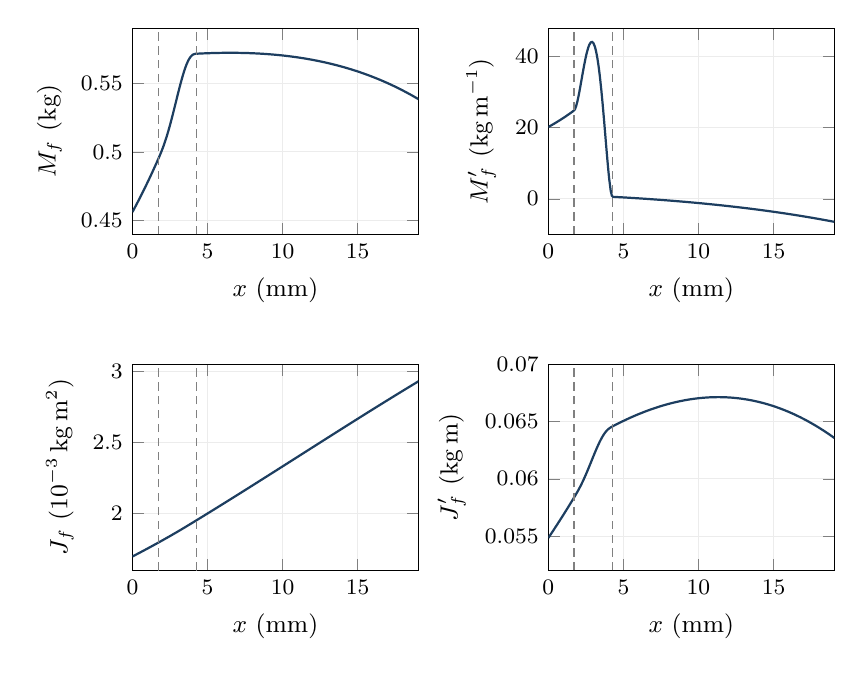
\begin{tikzpicture}
\begin{groupplot}[group style={group size=2 by 2,horizontal sep=1.65cm,vertical sep=1.65cm},width=.43\textwidth,height=4.2cm,xmin=0,xmax=19.05,xlabel={$x\ (\mathrm{mm})$},tick label style={font=\footnotesize},label style={font=\small},grid=major,grid style={gray!15},scaled ticks=false]
\nextgroupplot[ylabel={$M_f\ (\mathrm{kg})$},ymin=0.44,ymax=0.59]
\addplot[linkblue,thick,no marks] coordinates {(0.0000000,0.4562183) (0.1488281,0.4592522) (0.2976563,0.4623392) (0.4464844,0.4654807) (0.5953125,0.4686779) (0.7441406,0.4719324) (0.8929688,0.4752456) (1.0417969,0.4786190) (1.1906250,0.4820542) (1.3394531,0.4855528) (1.4882812,0.4891166) (1.5000000,0.4894000) (1.5882353,0.4915475) (1.6371094,0.4927472) (1.6764706,0.4937188) (1.7647059,0.4959165) (1.7859375,0.4964520) (1.8529412,0.4981719) (1.9347656,0.5003563) (1.9411765,0.5005322) (2.0294118,0.5030337) (2.0835937,0.5046511) (2.1176471,0.5057016) (2.2058824,0.5085506) (2.2324219,0.5094440) (2.2941176,0.5115863) (2.3812500,0.5147644) (2.3823529,0.5148057) (2.4705882,0.5181984) (2.5300781,0.5205753) (2.5588235,0.5217473) (2.6470588,0.5254291) (2.6789063,0.5267853) (2.7352941,0.5292155) (2.8235294,0.5330731) (2.8277344,0.5332581) (2.9117647,0.5369647) (2.9765625,0.5398205) (3.0000000,0.5408491) (3.0882353,0.5446822) (3.1253906,0.5462697) (3.1764706,0.5484173) (3.2647059,0.5520062) (3.2742188,0.5523824) (3.3529412,0.5554004) (3.4230469,0.5579264) (3.4411765,0.5585518) (3.5294118,0.5614149) (3.5718750,0.5626777) (3.6176471,0.5639488) (3.7058824,0.5661196) (3.7207031,0.5664468) (3.7941176,0.5679039) (3.8695313,0.5691147) (3.8823529,0.5692919) (3.9705882,0.5702923) (4.0183594,0.5706823) (4.0588235,0.5709365) (4.1470588,0.5712832) (4.1671875,0.5713293) (4.2352941,0.5714227) (4.3160156,0.5714736) (4.3235294,0.5714779) (4.4117647,0.5715271) (4.4648438,0.5715559) (4.5000000,0.5715745) (4.6136719,0.5716329) (4.7625000,0.5717047) (4.9113281,0.5717711) (5.0601563,0.5718321) (5.2089844,0.5718875) (5.3578125,0.5719374) (5.5066406,0.5719815) (5.6554687,0.5720199) (5.8042969,0.5720525) (5.9531250,0.5720791) (6.1019531,0.5720997) (6.2507813,0.5721141) (6.3996094,0.5721224) (6.5484375,0.5721244) (6.6972656,0.5721200) (6.8460938,0.5721091) (6.9949219,0.5720916) (7.1437500,0.5720675) (7.2925781,0.5720366) (7.4414062,0.5719989) (7.5902344,0.5719542) (7.7390625,0.5719025) (7.8878906,0.5718436) (8.0367188,0.5717775) (8.1855469,0.5717041) (8.3343750,0.5716232) (8.4832031,0.5715348) (8.6320313,0.5714388) (8.7808594,0.5713350) (8.9296875,0.5712233) (9.0785156,0.5711037) (9.2273438,0.5709760) (9.3761719,0.5708402) (9.5250000,0.5706961) (9.6738281,0.5705436) (9.8226563,0.5703826) (9.9714844,0.5702129) (10.1203125,0.5700346) (10.2691406,0.5698474) (10.4179688,0.5696513) (10.5667969,0.5694461) (10.7156250,0.5692317) (10.8644531,0.5690080) (11.0132813,0.5687749) (11.1621094,0.5685322) (11.3109375,0.5682799) (11.4597656,0.5680178) (11.6085938,0.5677458) (11.7574219,0.5674637) (11.9062500,0.5671715) (12.0550781,0.5668690) (12.2039063,0.5665560) (12.3527344,0.5662326) (12.5015625,0.5658984) (12.6503906,0.5655534) (12.7992188,0.5651975) (12.9480469,0.5648305) (13.0968750,0.5644522) (13.2457031,0.5640627) (13.3945313,0.5636616) (13.5433594,0.5632489) (13.6921875,0.5628244) (13.8410156,0.5623880) (13.9898438,0.5619395) (14.1386719,0.5614789) (14.2875000,0.5610058) (14.4363281,0.5605203) (14.5851563,0.5600222) (14.7339844,0.5595112) (14.8828125,0.5589873) (15.0316406,0.5584503) (15.1804688,0.5579000) (15.3292969,0.5573364) (15.4781250,0.5567591) (15.6269531,0.5561682) (15.7757813,0.5555633) (15.9246094,0.5549445) (16.0734375,0.5543114) (16.2222656,0.5536639) (16.3710938,0.5530020) (16.5199219,0.5523253) (16.6687500,0.5516338) (16.8175781,0.5509272) (16.9664062,0.5502055) (17.1152344,0.5494684) (17.2640625,0.5487157) (17.4128906,0.5479473) (17.5617188,0.5471631) (17.7105469,0.5463628) (17.8593750,0.5455462) (18.0082031,0.5447133) (18.1570312,0.5438637) (18.3058594,0.5429974) (18.4546875,0.5421141) (18.6035156,0.5412137) (18.7523438,0.5402960) (18.9011719,0.5393608) (19.0500000,0.5384079)};
\draw[densely dashed,gray] (axis cs:1.7131461765058746,0.44)--(axis cs:1.7131461765058746,0.59);
\draw[densely dashed,gray] (axis cs:4.282930952656586,0.44)--(axis cs:4.282930952656586,0.59);
\nextgroupplot[ylabel={$M_f^\prime\ (\mathrm{kg\,m^{-1}})$},ymin=-10,ymax=48]
\addplot[linkblue,thick,no marks] coordinates {(0.0000000,20.2098358) (0.1488281,20.5622654) (0.2976563,20.9234821) (0.4464844,21.2937838) (0.5953125,21.6734809) (0.7441406,22.0628972) (0.8929688,22.4623706) (1.0417969,22.8722538) (1.1906250,23.2929148) (1.3394531,23.7247385) (1.4882812,24.1681266) (1.5000000,24.2035424) (1.5882353,24.4726099) (1.6371094,24.6234992) (1.6764706,24.7459925) (1.7647059,25.1362491) (1.7859375,25.3117718) (1.8529412,26.0763180) (1.9347656,27.3766040) (1.9411765,27.4927113) (2.0294118,29.2556593) (2.0835937,30.4570316) (2.1176471,31.2435341) (2.2058824,33.3448180) (2.2324219,33.9836347) (2.2941176,35.4587725) (2.3812500,37.4705693) (2.3823529,37.4952080) (2.4705882,39.3737156) (2.5300781,40.5147375) (2.5588235,41.0226566) (2.6470588,42.3781354) (2.6789063,42.7840820) (2.7352941,43.3831263) (2.8235294,43.9868791) (2.8277344,44.0048490) (2.9117647,44.1446979) (2.9765625,43.9540522) (3.0000000,43.8181744) (3.0882353,42.9759460) (3.1253906,42.4611048) (3.1764706,41.5950533) (3.2647059,39.6629690) (3.2742188,39.4216357) (3.3529412,37.1803730) (3.4230469,34.8263291) (3.4411765,34.1647363) (3.5294118,30.6547504) (3.5718750,28.8074138) (3.6176471,26.7155777) (3.7058824,22.4447977) (3.7207031,21.7039460) (3.7941176,17.9787520) (3.8695313,14.1423004) (3.8823529,13.4987396) (3.9705882,9.2361710) (4.0183594,7.1174804) (4.0588235,5.4753789) (4.1470588,2.5523800) (4.1671875,2.0417851) (4.2352941,0.8476509) (4.3160156,0.5697875) (4.3235294,0.5680520) (4.4117647,0.5475711) (4.4648438,0.5351604) (4.5000000,0.5269029) (4.6136719,0.4999987) (4.7625000,0.4642975) (4.9113281,0.4280514) (5.0601563,0.3912555) (5.2089844,0.3539044) (5.3578125,0.3159928) (5.5066406,0.2775154) (5.6554687,0.2384667) (5.8042969,0.1988414) (5.9531250,0.1586339) (6.1019531,0.1178385) (6.2507813,0.0764498) (6.3996094,0.0344619) (6.5484375,-0.0081310) (6.6972656,-0.0513345) (6.8460938,-0.0951546) (6.9949219,-0.1395973) (7.1437500,-0.1846685) (7.2925781,-0.2303743) (7.4414062,-0.2767209) (7.5902344,-0.3237143) (7.7390625,-0.3713609) (7.8878906,-0.4196669) (8.0367188,-0.4686388) (8.1855469,-0.5182829) (8.3343750,-0.5686058) (8.4832031,-0.6196140) (8.6320313,-0.6713140) (8.7808594,-0.7237127) (8.9296875,-0.7768167) (9.0785156,-0.8306328) (9.2273438,-0.8851680) (9.3761719,-0.9404290) (9.5250000,-0.9964230) (9.6738281,-1.0531570) (9.8226563,-1.1106380) (9.9714844,-1.1688733) (10.1203125,-1.2278700) (10.2691406,-1.2876355) (10.4179688,-1.3481772) (10.5667969,-1.4095024) (10.7156250,-1.4716186) (10.8644531,-1.5345334) (11.0132813,-1.5982543) (11.1621094,-1.6627890) (11.3109375,-1.7281452) (11.4597656,-1.7943306) (11.6085938,-1.8613531) (11.7574219,-1.9292205) (11.9062500,-1.9979407) (12.0550781,-2.0675218) (12.2039063,-2.1379716) (12.3527344,-2.2092984) (12.5015625,-2.2815102) (12.6503906,-2.3546152) (12.7992188,-2.4286216) (12.9480469,-2.5035376) (13.0968750,-2.5793715) (13.2457031,-2.6561317) (13.3945313,-2.7338265) (13.5433594,-2.8124643) (13.6921875,-2.8920536) (13.8410156,-2.9726028) (13.9898438,-3.0541203) (14.1386719,-3.1366148) (14.2875000,-3.2200948) (14.4363281,-3.3045687) (14.5851563,-3.3900452) (14.7339844,-3.4765329) (14.8828125,-3.5640403) (15.0316406,-3.6525760) (15.1804688,-3.7421486) (15.3292969,-3.8327667) (15.4781250,-3.9244389) (15.6269531,-4.0171738) (15.7757813,-4.1109798) (15.9246094,-4.2058656) (16.0734375,-4.3018396) (16.2222656,-4.3989103) (16.3710938,-4.4970862) (16.5199219,-4.5963755) (16.6687500,-4.6967866) (16.8175781,-4.7983279) (16.9664062,-4.9010074) (17.1152344,-5.0048334) (17.2640625,-5.1098140) (17.4128906,-5.2159569) (17.5617188,-5.3232703) (17.7105469,-5.4317617) (17.8593750,-5.5414389) (18.0082031,-5.6523094) (18.1570312,-5.7643807) (18.3058594,-5.8776599) (18.4546875,-5.9921542) (18.6035156,-6.1078706) (18.7523438,-6.2248158) (18.9011719,-6.3429964) (19.0500000,-6.4624188)};
\draw[densely dashed,gray] (axis cs:1.7131461765058746,-10)--(axis cs:1.7131461765058746,48);
\draw[densely dashed,gray] (axis cs:4.282930952656586,-10)--(axis cs:4.282930952656586,48);
\nextgroupplot[ylabel={$J_f\ (10^{-3}\,\mathrm{kg\,m^2})$},ymin=1.6,ymax=3.05]
\addplot[linkblue,thick,no marks] coordinates {(0.0000000,1.6983262) (0.1488281,1.7065100) (0.2976563,1.7147374) (0.4464844,1.7230087) (0.5953125,1.7313244) (0.7441406,1.7396848) (0.8929688,1.7480904) (1.0417969,1.7565416) (1.1906250,1.7650389) (1.3394531,1.7735828) (1.4882812,1.7821737) (1.5000000,1.7828522) (1.5882353,1.7879701) (1.6371094,1.7908121) (1.6764706,1.7931048) (1.7647059,1.7982564) (1.7859375,1.7994985) (1.8529412,1.8034251) (1.9347656,1.8082339) (1.9411765,1.8086113) (2.0294118,1.8138156) (2.0835937,1.8170207) (2.1176471,1.8190388) (2.2058824,1.8242818) (2.2324219,1.8258628) (2.2941176,1.8295455) (2.3812500,1.8347646) (2.3823529,1.8348308) (2.4705882,1.8401386) (2.5300781,1.8437303) (2.5588235,1.8454697) (2.6470588,1.8508247) (2.6789063,1.8527636) (2.7352941,1.8562044) (2.8235294,1.8616090) (2.8277344,1.8618672) (2.9117647,1.8670388) (2.9765625,1.8710424) (3.0000000,1.8724938) (3.0882353,1.8779738) (3.1253906,1.8802888) (3.1764706,1.8834784) (3.2647059,1.8890069) (3.2742188,1.8896043) (3.3529412,1.8945583) (3.4230469,1.8989848) (3.4411765,1.9001317) (3.5294118,1.9057255) (3.5718750,1.9084244) (3.6176471,1.9113382) (3.7058824,1.9169681) (3.7207031,1.9179153) (3.7941176,1.9226132) (3.8695313,1.9274485) (3.8823529,1.9282715) (3.9705882,1.9339410) (4.0183594,1.9370146) (4.0588235,1.9396199) (4.1470588,1.9453065) (4.1671875,1.9466047) (4.2352941,1.9509994) (4.3160156,1.9562124) (4.3235294,1.9566979) (4.4117647,1.9624017) (4.4648438,1.9658354) (4.5000000,1.9681108) (4.6136719,1.9754734) (4.7625000,1.9851260) (4.9113281,1.9947930) (5.0601563,2.0044741) (5.2089844,2.0141691) (5.3578125,2.0238775) (5.5066406,2.0335992) (5.6554687,2.0433339) (5.8042969,2.0530812) (5.9531250,2.0628410) (6.1019531,2.0726128) (6.2507813,2.0823964) (6.3996094,2.0921914) (6.5484375,2.1019977) (6.6972656,2.1118148) (6.8460938,2.1216425) (6.9949219,2.1314805) (7.1437500,2.1413284) (7.2925781,2.1511859) (7.4414062,2.1610528) (7.5902344,2.1709287) (7.7390625,2.1808132) (7.8878906,2.1907061) (8.0367188,2.2006071) (8.1855469,2.2105158) (8.3343750,2.2204318) (8.4832031,2.2303549) (8.6320313,2.2402847) (8.7808594,2.2502209) (8.9296875,2.2601632) (9.0785156,2.2701111) (9.2273438,2.2800644) (9.3761719,2.2900228) (9.5250000,2.2999858) (9.6738281,2.3099531) (9.8226563,2.3199244) (9.9714844,2.3298994) (10.1203125,2.3398776) (10.2691406,2.3498588) (10.4179688,2.3598425) (10.5667969,2.3698285) (10.7156250,2.3798162) (10.8644531,2.3898055) (11.0132813,2.3997959) (11.1621094,2.4097870) (11.3109375,2.4197786) (11.4597656,2.4297701) (11.6085938,2.4397613) (11.7574219,2.4497518) (11.9062500,2.4597412) (12.0550781,2.4697291) (12.2039063,2.4797152) (12.3527344,2.4896990) (12.5015625,2.4996802) (12.6503906,2.5096584) (12.7992188,2.5196333) (12.9480469,2.5296043) (13.0968750,2.5395713) (13.2457031,2.5495337) (13.3945313,2.5594912) (13.5433594,2.5694433) (13.6921875,2.5793898) (13.8410156,2.5893301) (13.9898438,2.5992640) (14.1386719,2.6091909) (14.2875000,2.6191106) (14.4363281,2.6290226) (14.5851563,2.6389265) (14.7339844,2.6488220) (14.8828125,2.6587085) (15.0316406,2.6685857) (15.1804688,2.6784533) (15.3292969,2.6883108) (15.4781250,2.6981577) (15.6269531,2.7079938) (15.7757813,2.7178185) (15.9246094,2.7276315) (16.0734375,2.7374324) (16.2222656,2.7472207) (16.3710938,2.7569961) (16.5199219,2.7667581) (16.6687500,2.7765064) (16.8175781,2.7862405) (16.9664062,2.7959599) (17.1152344,2.8056644) (17.2640625,2.8153534) (17.4128906,2.8250266) (17.5617188,2.8346835) (17.7105469,2.8443238) (17.8593750,2.8539470) (18.0082031,2.8635527) (18.1570312,2.8731405) (18.3058594,2.8827099) (18.4546875,2.8922606) (18.6035156,2.9017921) (18.7523438,2.9113041) (18.9011719,2.9207961) (19.0500000,2.9302676)};
\draw[densely dashed,gray] (axis cs:1.7131461765058746,1.6)--(axis cs:1.7131461765058746,3.05);
\draw[densely dashed,gray] (axis cs:4.282930952656586,1.6)--(axis cs:4.282930952656586,3.05);
\nextgroupplot[ylabel={$J_f^\prime\ (\mathrm{kg\,m})$},ymin=0.052,ymax=0.07,yticklabel style={/pgf/number format/fixed,/pgf/number format/precision=3}]
\addplot[linkblue,thick,no marks] coordinates {(0.0000000,0.0548435) (0.1488281,0.0551345) (0.2976563,0.0554282) (0.4464844,0.0557247) (0.5953125,0.0560240) (0.7441406,0.0563262) (0.8929688,0.0566314) (1.0417969,0.0569395) (1.1906250,0.0572508) (1.3394531,0.0575652) (1.4882812,0.0578827) (1.5000000,0.0579079) (1.5882353,0.0580978) (1.6371094,0.0582036) (1.6764706,0.0582890) (1.7647059,0.0584814) (1.7859375,0.0585280) (1.8529412,0.0586769) (1.9347656,0.0588635) (1.9411765,0.0588784) (2.0294118,0.0590878) (2.0835937,0.0592211) (2.1176471,0.0593068) (2.2058824,0.0595360) (2.2324219,0.0596070) (2.2941176,0.0597757) (2.3812500,0.0600226) (2.3823529,0.0600258) (2.4705882,0.0602855) (2.5300781,0.0604655) (2.5588235,0.0605538) (2.6470588,0.0608293) (2.6789063,0.0609302) (2.7352941,0.0611103) (2.8235294,0.0613948) (2.8277344,0.0614084) (2.9117647,0.0616807) (2.9765625,0.0618902) (3.0000000,0.0619656) (3.0882353,0.0622469) (3.1253906,0.0623637) (3.1764706,0.0625221) (3.2647059,0.0627884) (3.2742188,0.0628164) (3.3529412,0.0630430) (3.4230469,0.0632353) (3.4411765,0.0632834) (3.5294118,0.0635069) (3.5718750,0.0636078) (3.6176471,0.0637114) (3.7058824,0.0638950) (3.7207031,0.0639237) (3.7941176,0.0640564) (3.8695313,0.0641762) (3.8823529,0.0641950) (3.9705882,0.0643113) (4.0183594,0.0643656) (4.0588235,0.0644071) (4.1470588,0.0644857) (4.1671875,0.0645017) (4.2352941,0.0645520) (4.3160156,0.0646079) (4.3235294,0.0646131) (4.4117647,0.0646733) (4.4648438,0.0647092) (4.5000000,0.0647328) (4.6136719,0.0648086) (4.7625000,0.0649061) (4.9113281,0.0650018) (5.0601563,0.0650956) (5.2089844,0.0651875) (5.3578125,0.0652775) (5.5066406,0.0653656) (5.6554687,0.0654517) (5.8042969,0.0655359) (5.9531250,0.0656180) (6.1019531,0.0656982) (6.2507813,0.0657764) (6.3996094,0.0658526) (6.5484375,0.0659267) (6.6972656,0.0659987) (6.8460938,0.0660687) (6.9949219,0.0661366) (7.1437500,0.0662024) (7.2925781,0.0662661) (7.4414062,0.0663277) (7.5902344,0.0663871) (7.7390625,0.0664444) (7.8878906,0.0664995) (8.0367188,0.0665524) (8.1855469,0.0666031) (8.3343750,0.0666516) (8.4832031,0.0666978) (8.6320313,0.0667418) (8.7808594,0.0667836) (8.9296875,0.0668231) (9.0785156,0.0668603) (9.2273438,0.0668952) (9.3761719,0.0669278) (9.5250000,0.0669580) (9.6738281,0.0669860) (9.8226563,0.0670115) (9.9714844,0.0670348) (10.1203125,0.0670556) (10.2691406,0.0670740) (10.4179688,0.0670901) (10.5667969,0.0671037) (10.7156250,0.0671149) (10.8644531,0.0671237) (11.0132813,0.0671300) (11.1621094,0.0671338) (11.3109375,0.0671352) (11.4597656,0.0671341) (11.6085938,0.0671305) (11.7574219,0.0671244) (11.9062500,0.0671157) (12.0550781,0.0671045) (12.2039063,0.0670908) (12.3527344,0.0670746) (12.5015625,0.0670557) (12.6503906,0.0670344) (12.7992188,0.0670104) (12.9480469,0.0669838) (13.0968750,0.0669546) (13.2457031,0.0669229) (13.3945313,0.0668885) (13.5433594,0.0668514) (13.6921875,0.0668118) (13.8410156,0.0667694) (13.9898438,0.0667245) (14.1386719,0.0666768) (14.2875000,0.0666265) (14.4363281,0.0665736) (14.5851563,0.0665179) (14.7339844,0.0664595) (14.8828125,0.0663985) (15.0316406,0.0663347) (15.1804688,0.0662682) (15.3292969,0.0661990) (15.4781250,0.0661271) (15.6269531,0.0660524) (15.7757813,0.0659750) (15.9246094,0.0658949) (16.0734375,0.0658120) (16.2222656,0.0657264) (16.3710938,0.0656380) (16.5199219,0.0655468) (16.6687500,0.0654529) (16.8175781,0.0653562) (16.9664062,0.0652567) (17.1152344,0.0651544) (17.2640625,0.0650494) (17.4128906,0.0649416) (17.5617188,0.0648310) (17.7105469,0.0647176) (17.8593750,0.0646014) (18.0082031,0.0644824) (18.1570312,0.0643607) (18.3058594,0.0642361) (18.4546875,0.0641088) (18.6035156,0.0639786) (18.7523438,0.0638457) (18.9011719,0.0637099) (19.0500000,0.0635714)};
\draw[densely dashed,gray] (axis cs:1.7131461765058746,0.052)--(axis cs:1.7131461765058746,0.07);
\draw[densely dashed,gray] (axis cs:4.282930952656586,0.052)--(axis cs:4.282930952656586,0.07);
\end{groupplot}
\end{tikzpicture}
\caption{Exact contact-map values for the v1.1.5 reference geometry and simplified mass model. Dashed vertical lines mark the sheave positions corresponding to the two ramp-profile junctions. The same profile-coordinate spans map to different sheave-travel spans.}
\label{fig:maps}
\end{figure}

\section{What was checked, and what each check establishes}
\label{sec:verification}

The companion separates errors in the physical reconstruction from changes introduced by the interface and from the existing interpolation approximation. This is necessary because equal-looking force curves could conceal an omitted shaft inertia, an inconsistent derivative, or a changed contact branch.

\subsection{Independent checks of the physical construction}

A straight ramp provides a closed-form angle and its derivatives, derived in Appendix~\ref{app:straight}. Across 41 positions, the maximum absolute differences from the implicit construction were $6.11\times10^{-16}$ rad in $q_f$, $2.14\times10^{-14}\,\mathrm{m^{-1}}$ in $q_f'$, and $3.19\times10^{-12}\,\mathrm{m^{-2}}$ in $q_f''$.

The mass formulas were also compared with explicit material-point sums for a reflected three-dimensional point cloud with nonzero $v$ offsets, circumferential spread, and product moment $S_{uv}$. Direct particle accelerations and angular momentum supplied a separate Newtonian force/torque check over 57 states. The maximum force difference was $1.37\times10^{-12}\,\mathrm{N}$, and the maximum power-balance residual was $4.55\times10^{-13}\,\mathrm{W}$. The per-roller force projection also satisfied the pivot moment balance. These tests exercise more than the special slender-arm algebra.

For the actual $C^3$ reference profile, the independent exact map was compared with CINDER's exact evaluator at 71 positions, including both sides of each profile junction. The observed map differences were
\begin{center}
\begin{tabular}{@{}lll@{}}
\toprule
Quantity & Maximum absolute difference & Units\\
\midrule
$M_f$ & $2.48\times10^{-13}$ & $\mathrm{kg}$\\
$M_f'$ & $6.28\times10^{-10}$ & $\mathrm{kg\,m^{-1}}$\\
$J_f$ & $1.56\times10^{-15}$ & $\mathrm{kg\,m^2}$\\
$J_f'$ & $1.42\times10^{-14}$ & $\mathrm{kg\,m}$\\
\bottomrule
\end{tabular}
\end{center}
These differences include the separate numerical root solves. They support agreement of the implemented geometry and inertia construction; they are not experimental validation of the chosen dimensions or mass approximation.

\subsection{A test of the interface alone}

For this comparison, the four-map provider was formed from the existing runtime sample, preserving its angle spline and mass properties. The new element was then compared with the original fixed-pivot force element.

\begin{center}
\begin{tabularx}{\textwidth}{@{}YP{.25\textwidth}P{.23\textwidth}@{}}
\toprule
Compared behavior & Coverage & Observed difference\\
\midrule
Affine force and torque biases and all closure gains & 390 local contexts; both owning shafts & Zero at sampled contexts\\[.4em]
Local kinetic matrix and compressive-contact margin & Same 390 contexts & Zero at sampled contexts\\[.4em]
Contact transition through zero reaction & Positive, zero, negative cases & Same sign and zero guard\\[.4em]
Engaged algebraic closure & 12 paired solves; free shift and both stop rows & Same eight unknowns\\[.4em]
Free primary deadzone & 2 paired evaluations & Same accelerations\\[.4em]
Kinetic energy and upper-stop projection & Both velocity topologies; 1 paired impact & Same energy and successor state\\
\bottomrule
\end{tabularx}
\end{center}

The engaged comparisons are algebraic checks at frozen states, not a new campaign of admissible time trajectories. Their purpose is to check that the new representation reaches the listed continuous and event calculations. Equality of the continuous coefficients alone would not establish equality of the stop projection if the kinetic modes were omitted.

\subsection{Interpolation error remains a separate numerical approximation}

An independently compiled 257-node angle spline was compared with its exact contact construction at 1,027 positions, including the two profile-junction closures. The sampled maximum absolute differences were
\begin{center}
\begin{tabular}{@{}lll@{}}
\toprule
Quantity & Compiled versus exact difference & Units\\
\midrule
$M_f$ & $6.60\times10^{-7}$ & $\mathrm{kg}$\\
$M_f'$ & $9.26\times10^{-2}$ & $\mathrm{kg\,m^{-1}}$\\
$J_f$ & $9.38\times10^{-13}$ & $\mathrm{kg\,m^2}$\\
$J_f'$ & $3.73\times10^{-8}$ & $\mathrm{kg\,m}$\\
\bottomrule
\end{tabular}
\end{center}
The derivative $M_f'$ is more sensitive because it contains the second derivative of the angle spline. A small pose error does not by itself certify an equally small acceleration-term error. Its force consequence at a particular state is assessed through
\begin{equation}
  |\delta F_{f,x}|\le\half|\delta J_f'|\omega^2
            +|\delta M_f|\,|\ddot x|
            +\half|\delta M_f'|\dot x^2,
  \label{eq:error-force}
\end{equation}
with an analogous torque estimate
\begin{equation}
  |\delta\tau_f|\le |\delta J_f|\,|\alpha|
                            +|\delta J_f'|\,|\dot x\omega|.
\end{equation}
The tabulated differences are sampled diagnostics, not rigorous bounds over all positions. They also belong to the spline approximation, not to the change of mechanical interface. The interface comparison above deliberately preserved the same spline so that these two issues remain distinguishable.

\section{Relationship to the sliding-block implementation}
\label{sec:next}

A fixed pivot removes translation of the attachment from the relative motion:
its effective mass follows directly from the angular motion ratio and pivot
inertia. The sliding-block mechanism has no such pivot. Both COM coordinates
translate, and the guide must supply the force and moment needed to preserve
orientation. The \href{../sliding_block/formulation.pdf}{sliding-block document}
constructs those quantities from two finite contact profiles. Their equality of
interface does not imply equality of internal reactions or impact feasibility.

The production regression in
\texttt{test/smoke/test\_centrifugal\_inertia\_boundary.py} compares the retained
fixed-pivot laws with the common evaluator, including both shaft channels,
closure gains, stored energy, impact projection, and a ten-second launch with
belt engagement and the upper travel stop. This supplements the historical
reference comparisons below without changing their recorded provenance.

\clearpage
\appendix
\section{Constructing the reference ramp profile}
\label{app:profile}

All local segment heights below start at zero. Their placement in the complete ramp adds the accumulated heights of the preceding segments, preserving position continuity. The profile coordinate runs over a $5\,\mathrm{mm}$ straight segment, a $3\,\mathrm{mm}$ transition, and a $30\,\mathrm{mm}$ circular segment.

\subsection{Straight and circular segments}

For the initial straight portion, at local coordinate $\eta$,
\begin{equation}
  h_L(\eta)=\eta\tan35^\circ,\qquad
  h_L'=\tan35^\circ,\qquad h_L''=h_L'''=0.
\end{equation}
Primes within this appendix denote local segment-coordinate derivatives. For the circular part, let $\alpha_0=35^\circ$, $\alpha_1=20^\circ$, and $\ell_C=30\,\mathrm{mm}$. Its radius and a convenient local variable are
\begin{equation}
  R_C=\frac{\ell_C}{\sin\alpha_0-\sin\alpha_1},
  \qquad u(\eta)=\sin\alpha_0-\frac{\eta}{R_C}.
\end{equation}
The profile and derivatives are
\begin{align}
  h_C&=R_C\left[\sqrt{1-u^2}-\cos\alpha_0\right],\notag\\
  h_C'&=\frac{u}{\sqrt{1-u^2}},\qquad
  h_C''=-\frac{1}{R_C(1-u^2)^{3/2}},\qquad
  h_C'''=\frac{3u}{R_C^2(1-u^2)^{5/2}}.
  \label{eq:circular-profile}
\end{align}
The slope decreases from $\tan\alpha_0$ to $\tan\alpha_1$. Although the straight and circular portions begin with the same slope, their second derivatives do not match. Joining them directly would therefore not give the smoothness required by the finite-roller acceleration map.

\subsection{A transition that matches derivatives through third order}

Let $\ell_B=3\,\mathrm{mm}$ and $v=\eta/\ell_B$. Represent the transition's slope as a quintic
\begin{equation}
  h_B'(\eta)=P(v)=\sum_{i=0}^{5}a_iv^i.
\end{equation}
To make the height $C^3$, match its first three derivatives at both ends. If the required endpoint values are $(p_L,k_L,t_L)$ and $(p_R,k_R,t_R)$, then
\begin{align}
 P(0)&=p_L,& P'(0)&=\ell_Bk_L,&P''(0)&=\ell_B^2t_L,\notag\\
 P(1)&=p_R,& P'(1)&=\ell_Bk_R,&P''(1)&=\ell_B^2t_R.
 \label{eq:blend-conditions}
\end{align}
The derivatives of $P$ here are with respect to its dimensionless argument $v$. Take the left data from the end of the straight segment and the right data from the start of the circle. A direct coefficient construction is
\begin{align}
 a_0&=p_L,&a_1&=\ell_Bk_L,&a_2&=\half\ell_B^2t_L,\notag\\
 b_0&=p_R-a_0-a_1-a_2,\notag\\
 b_1&=\ell_Bk_R-a_1-2a_2,\qquad
 b_2=\ell_B^2t_R-2a_2,\notag\\
 a_3&=10b_0-4b_1+\half b_2,\notag\\
 a_4&=-15b_0+7b_1-b_2,\qquad
 a_5=6b_0-3b_1+\half b_2.
 \label{eq:blend-coefficients}
\end{align}
Integrating the slope produces the sixth-degree local height:
\begin{equation}
 h_B(\eta)=\ell_B\sum_{i=0}^{5}\frac{a_i}{i+1}v^{i+1}.
\end{equation}
The resulting end height sets the circular segment's radial placement. This construction specifies endpoint derivatives rather than independently fixing an incompatible endpoint height.

The reference code represents this same quintic slope in a Bernstein basis using endpoint Hermite data, then integrates it. The production v1.1.5 routine evaluates its polynomial from the nearer endpoint and returns the exact endpoint constraints when evaluated at an endpoint. Both choices address cancellation in short segments; neither changes the intended profile. The $3\,\mathrm{mm}$ smoothing length itself is a model approximation and remains distinct from these numerical evaluation choices.

\section{A straight-ramp solution for an independent check}
\label{app:straight}

A finite roller on a straight ramp admits an explicit solution, which can test the implicit derivatives without using the same contact solver as the reference. Set $d=-1$, $\sigma=+1$, and $h(\xi)=k\xi$ with $k>0$. The surface line and centre-offset line satisfy
\begin{equation}
  r_K+kX_K=r_A+k(X_A+x),
  \qquad
  r_C+kX_C=r_A+k(X_A+x)-R_{\mathrm{roll}}\sqrt{1+k^2}.
\end{equation}
Substituting the arm-circle coordinates gives
\begin{equation}
  L_f(\sin q_f+k\cos q_f)
    =(r_A-r_P)+k(X_A-X_P+x)-R_{\mathrm{roll}}\sqrt{1+k^2}.
\end{equation}
Let $\gamma=\arctan k$, $w=\sqrt{1+k^2}$, and call the right-hand side $D(x)$. Since $\sin q_f+k\cos q_f=w\sin(q_f+\gamma)$, the selected branch is
\begin{equation}
  q_f=\arcsin\!\left(\frac{D}{L_fw}\right)-\gamma,
  \qquad \cos(q_f+\gamma)>0.
\end{equation}
Its derivatives are
\begin{equation}
  q_f'=\frac{k}{L_fw\cos(q_f+\gamma)},
  \qquad q_f''=(q_f')^2\tan(q_f+\gamma).
\end{equation}
The test uses the reference dimensions with a $35^\circ$ straight profile, restricting the physical profile to $0\le\xi\le15\,\mathrm{mm}$ and sheave travel to $0\le x\le7\,\mathrm{mm}$. This stays on the stated regular branch. It checks the roller-radius offset, angle convention, and both derivatives against closed-form expressions.

\clearpage
\section{Running and extending the companion reference}
\label{app:running}

The adjacent \texttt{reference/} directory contains \texttt{fixed\_pivot\_reference.py}, \texttt{verify\_reference.py}, a short README, and the result record used for the original reference comparison. The first module has no CINDER imports. It constructs the reference profile, contact geometry, mass moments, exact inertia maps, and optional compiled angle map. Its monotone forward-arm solver is deliberately limited to the admitted reference branch; it does not replace the production geometry audit for arbitrary user-defined ramps.

The verification script requires Python, NumPy, and SciPy. Run the independent checks with
\begin{lstlisting}[language={}]
python verify_reference.py
\end{lstlisting}
To include the pinned CINDER comparison, provide a checkout whose \texttt{cvtModel} content matches v1.1.5:
\begin{lstlisting}[language={}]
python verify_reference.py --repo /path/to/CVT-Simulator
\end{lstlisting}
The script verifies the source match and does not edit the repository. It writes its JSON results beside the script unless an alternative \texttt{--output} path is supplied. The recorded run used Python 3.12.14, NumPy 2.3.5, and SciPy 1.17.0. The model source matches commit \texttt{8261226b8cd1}; the inspected repository head was \texttt{a2dcdc66a965} with unchanged \texttt{cvtModel} content.

The production adaptation preserves the existing contact builder and spline and exposes \cref{eq:four-maps} through the shared provider. The adjacent companion remains pinned to v1.1.5 for reproduction of the historical tables; the current smoke suite tests the 1.2.0 implementation and its coupled behavior.

\clearpage
\begingroup\raggedright
\begin{thebibliography}{9}
\addcontentsline{toc}{section}{References}
\bibitem{formulation}
Kai Arseneau and W. Spencer Smith.
\emph{A First-Principles Dynamic Model of a Rubber V-Belt CVT for General Transient Simulation: With Mechanical Actuation and Traction-Limited Torque Transfer}.
Supplied manuscript, October 1, 2026. Section 3.2.1 and Appendix A.

\bibitem{general}
\emph{General Centrifugal Mechanisms: From Compatible Motion to Clamping Force and Shaft Coupling}.
CINDER technical note, Revision 4, October 9, 2026; canonical 1.2.0 edition.
\href{../common_boundary/formulation.pdf}{Companion common-boundary document}.

\bibitem{implementation}
CINDER v1.1.5, \texttt{gr812b/CVT-Simulator}, commit \texttt{8261226b8cd1e8b65c883d3a382c3f109ccbb10c}.
\href{https://github.com/gr812b/CVT-Simulator/blob/8261226b8cd1e8b65c883d3a382c3f109ccbb10c/cvtModel/src/cinder/model/cvt/actuation/fixed_pivot_flyweight.py}{Fixed-pivot geometry, mass moments, branch compilation, and runtime map};
\href{https://github.com/gr812b/CVT-Simulator/blob/8261226b8cd1e8b65c883d3a382c3f109ccbb10c/cvtModel/src/cinder/model/cvt/actuation/forces/fixed_pivot_flyweight.py}{force, torque, contact policy, and kinetic modes};
\href{https://github.com/gr812b/CVT-Simulator/blob/8261226b8cd1e8b65c883d3a382c3f109ccbb10c/cvtModel/src/cinder/model/cvt/actuation/types.py}{existing pulley-element interfaces}.

\bibitem{fixture}
CINDER v1.1.5 reference files:
\href{https://github.com/gr812b/CVT-Simulator/blob/8261226b8cd1e8b65c883d3a382c3f109ccbb10c/cvtModel/examples/baja_primary_fixed_pivot_geometry.json}{physical flyweight reference geometry};
\href{https://github.com/gr812b/CVT-Simulator/blob/8261226b8cd1e8b65c883d3a382c3f109ccbb10c/cvtModel/examples/baja_baseline_assembly.json}{complete baseline assembly};
\href{https://github.com/gr812b/CVT-Simulator/blob/8261226b8cd1e8b65c883d3a382c3f109ccbb10c/cvtModel/src/cinder/model/cvt/profiles/c3_transition_segment.py}{C3 transition implementation}.
\end{thebibliography}
\endgroup
\end{document}
